\chapter{Yoneda I: Internal vs. external}

This section marks the start of a long journey that ends in
the statement and proof of the famous Yoneda lemma in category theory (\todo).
As with any important concept in category theory, the Yoneda lemma
can be understood through a variety of perspectives. In these
notes we will explore a particular perspective that feels most
relevant to PL: the Yoneda lemma is a means of connecting
the ``internal'' to the ``external''.

Consider, for example, the case of product.
In the preceding sections, we have given you the definition of product
that is most commonly found in standard textbooks on category theory.
This definition has an ``internal'' character, because it defines
product in a category \(\calC\) purely in terms of
other objects and morphisms \emph{inside} of \(\calC\).

But there is another way to define product.
Think back to \cref{thm:calc-products},
which showed how to interpret a simple programming language
in an arbitrary category \(\calC\) with finite products.
The proof of \cref{thm:calc-products} gave a recipe
for interpreting each of the judgments of programming language
in \(\calC\). Following this recipe,
each of the typing rules became
\emph{functions on morphisms}. For example, the typing rule
\[
\inferrule*[right=T-Fst]{\Gamma \vdash M : A \pltimes B}{\Gamma \vdash \plfst{M} : A}
\]
for projecting out the first component of a pair
was interpreted as a function
\begin{align*}
  \{\text{morphisms \(\llbr\Gamma\) to \(\llbr{A\pltimes B}\)}\}
  \longrightarrow
  \{\text{morphisms \(\llbr\Gamma\) to \(\llbr{A}\)} \},
\end{align*}
namely the function
that sends interpretations of \(\llbr{M}\) to interpretations of \(\llbr{\plfst M}\).

It turns out that we can promote this recipe into a \emph{definition} for product.
In contrast to the textbook definition in terms of objects and morphisms
of \(\calC\), this definition characterizes the product in terms of \emph{functions} between
\emph{sets} of morphisms. This gives it an ``external'' character,
because it defines the product in terms of set-theoretic objects (sets and functions)
that live \emph{outside} of \(\calC\).

Of course, it will make no difference whether one chooses the internal
or the external definition of product: as we will see further down the line,
the Yoneda lemma implies that the two formulations are equivalent.
As a warm up to this abstract proof, this section will show
concretely how the equivalence works for the special case of products.

First, we must make precise what we mean by this ``external'' definition of product
that defines product in terms of functions on morphisms.
To formalize this idea of ``maps between morphisms'',
  it's useful to have the following definition that we've put off for a long time.

\begin{definition}[Hom-set]
  Let \(X\) and \(Y\) be objects of a category \(\calC\).
  The \emph{hom-set} of $\calC$ at $X$ and $Y$, 
  written \(\calC(X,Y)\),
  is the set of morphisms from \(X\) to \(Y\):
  \[
  \calC(X,Y) := \{f \mid \dom(f) = X, \cod(f) = Y\}.
  \]
\end{definition}
\marginnote{%
The word ``hom'' is an abbreviation of ``homomorphism'',
and the name hom-set comes from the fact many of the original motivating examples of categories
had morphisms that were homomorphisms between algebraic structures.
}
For example, \begin{itemize}
\item In the category of finite sets and set functions $\FinSet$, the
  hom-set $\FinSet(\{a,b\}, \{1, 2, 3\})$ is the set of all functions
  from $\{a,b\}$ to $\{1, 2, 3\}$.
\item Hom-sets can be empty. In the divisibility category $(\mathbb{N}, \preceq)$,
the hom-set $\mathbb{N}(3,4) = \emptyset$, while $\mathbb{N}(3, 6) = \{\top\}$.
\end{itemize}
This definition lets us state formally what it means for an inference rule
like \(\textsc{T-Fst}\) to denote a function from morphisms to morphisms.
We shall say that the interpretation of \(\textsc{T-Fst}\) is
a family of functions \((\mathsf{Fst}_\Gamma)_{\Gamma\in\calC}\),
indexed by the ambient context \(\Gamma\),
of the following type:
\[
\mathsf{Fst}_\Gamma : \calC(\Gamma, A \times B) \to \calC(\Gamma, A)
\]

%% Let's pause to inspect the unusual shape of this function.
%% First, observe that this is a function between two sets: this is \emph{not} a
%% morphism in the category $\calC$.  Second, it is a function between two sets of
%% morphisms with the same domain, $\Gamma$.  And third, the function is
%% \emph{indexed by $\Gamma$}, written with a subscript. We can visualize elements
%% of this family of ``$\mathsf{Fst}$-like morphisms'' as follows:
We can visualize this family of functions as follows:
\begin{equation}
  % https://tikzcd.yichuanshen.de/#N4Igdg9gJgpgziAXAbVABwnAlgFyxMJZABgBpiBdUkANwEMAbAVxiRAB12BxOgW17oB9AIwgAvqXSZc+QijLCqtRizace-IQCZxkkBmx4CRMlqX1mrRB258BggMy6ph2UWGlF1C6usBBAAJOPF54AIAhAOd9aSM5ZC1SM28VKxA-aIMZY3lSB3NUtgA6EvElGCgAc3giUAAzACcIXiQyEBwIJAcUyzZKkRBqBjoAIxgGAAVYt2ssMGxYaMbm1uoOpAAWajGwKC62nzS6gaHR8anXHJA5hdYJeqaWxA92zsRu5V7rfp1TscnplcblhFvcQMsni91ogtp9fODBL8QMN-hdsnJrvMQXc9BCkIlXl0evD+k4-udARjgaDcY98Ws3rCURTLlSsYtiUdHGUxEA
\begin{tikzcd}
  {\color{red} \Gamma_1} \arrow[rd, "f" description, color = red] \arrow[rrdd, "f'" description, bend left, color = red] &             &   \\
  {\color{blue}\Gamma_2} \arrow[r, "g" description, color = blue] \arrow[rrd, "g'" description, color = blue]              & A \times B  &   \\
  {\color{orange} \Gamma_3} \arrow[ru, "h" description, color = orange] \arrow[rr, "h'" description, color = orange]              &             & A \\
  ...                                                                               &             &  
  \end{tikzcd}
  \label{cd:indexed-fam}
\end{equation}
As an example of working with this function, we have that
$\mathsf{Fst}_{\Gamma_1}(f) = f'$.

In addition to the basic type shown above, we will also require that \(\mathsf{Fst}\)
be \emph{natural} in \(\Gamma\).
Intuitively, what this means is that \(\mathsf{Fst}\) is in a sense ``polymorphic in \(\Gamma\)''.
Just as polymorphic functions in System F
respect ``change of representation'' for the type variables that they are polymorphic over~\citep{reynolds1983types},
we will require that the family of functions \((\mathsf{Fst}_\Gamma)_{\Gamma\in\mathsf{Ob}(\calC)}\)
respect ``change of \(\Gamma\)''.
Concretely, this means that if any input \(f\) as shown in the pictue above is changed into \(f \circ s\) via some morphism
$s : \Gamma' \to \Gamma$,
it must be the case that \(\mathsf{Fst}_\Gamma(f)\) is changed into \(\mathsf{Fst}_{\Gamma'}(f\circ s)\)
via \(s\) too. Formally, the following \emph{naturality condition} must hold for any such \(f\) and \(s\):\marginnote{We will save a formal abstract definition
of naturality for \todo.}

%% There may be many morphisms that satisfy the type signature of $\mathsf{Fst}$,
%% but the key is that there are relatively few that are
%% \emph{invariant under the choice of $\Gamma$}. Concretely, if
%% there are is a morphism $s : \Gamma' \to \Gamma$ that relates $\Gamma'$ to $\Gamma$,

%% We will build towards the idea that there is some family of ``\textsf{Fst}-like
%% functions'' that ought to behave coherently for different choices of context
%% $\Gamma$.  The notion of coherence we need is stability under parallel substitution.

\begin{align*}
  \mathsf{Fst}_\Gamma(f) \circ s = \mathsf{Fst}_{\Gamma'}(f \circ s)
\end{align*}
Another intution for this condition comes from the requirement that the interpretation of a programming language
be \emph{stable under substitution}.
For instance, we know that
$\plfst{M}$ is invariant under substitution for some (possibly multi-way)
substitution $s$:
\begin{align*}
  (\plfst{M})[s] \equiv \plfst{(M[s])}
\end{align*}
This program equation corresponds directly to the naturality condition given above.

Applying the above analysis to the typing rule \textsc{T-Snd}
gives an analogous function for extracting the second component of a pair:
\begin{align*}
  &\inferrule
    {\Gamma \vdash M : A \pltimes B}
    {\Gamma \vdash \plsnd{M} : B}
    \rightsquigarrow
    \mathsf{Snd}_\Gamma : \calC(\Gamma, A \times B) \to \calC(\Gamma, B)
    \\
  &\text{such that }\forall s : \Gamma' \to \Gamma,
    \mathsf{Snd}_\Gamma(f)\circ s = \mathsf{Snd}_\Gamma(f \circ s)
\end{align*}
The rule \textsc{T-Pair} for forming pairs becomes a function
that takes in two morphisms and bundles them together into a morphism into the product:
\begin{align*}
  &\inferrule
    {\Gamma \vdash M : A \quad
      \Gamma \vdash N : B }
    {\Gamma \vdash \plpair{M}{N} : A \times B}
    \rightsquigarrow
    \mathsf{Pair}_\Gamma : \calC(\Gamma, A) \times \calC(\Gamma, B) 
    \to \calC(\Gamma, A \times B)
\\
   &\text{such that }\forall s : \Gamma' \to \Gamma,
    \mathsf{Pair}_\Gamma(f, g)\circ s = \mathsf{Pair}_\Gamma(f \circ s, g \circ s)
\end{align*}
Finally, the $\beta$ and $\eta$ laws become equations between nested applications of the functinos \(\mathsf{Fst}\), \(\mathsf{Snd}\),
and \(\mathsf{Pair}\).
\begin{align*}
  \inferrule
    {\Gamma \vdash M : A \quad
      \Gamma \vdash N : B }
    {\Gamma \vdash \plfst{\plpair{M}{N}} \equiv M}
    &\quad\rightsquigarrow\quad
    \mathsf{Fst}_\Gamma(\mathsf{Pair}_\Gamma(f,g)) = f
\\
  \inferrule
    {\Gamma \vdash M : A \quad
      \Gamma \vdash N : B }
    {\Gamma \vdash \plsnd{\plpair{M}{N}} \equiv N}
    &\quad\rightsquigarrow\quad
    \mathsf{Snd}_\Gamma(\mathsf{Pair}_\Gamma(f,g)) = g
\\
  \inferrule
    {\Gamma \vdash M : A \times B}
    {\Gamma \vdash M \equiv \plpair{\plfst{M}}{\plsnd{M}} \equiv N}
    &\quad\rightsquigarrow\quad
    \mathsf{Pair}_\Gamma(\mathsf{Fst}_\Gamma(f), \mathsf{Snd}_\Gamma(f)) = f
\end{align*}
Packaging up all of these constraints into a definition,\footnote{We have chosen to name this concept ``PL-product'' as it was derived from the typing rules for product types in a programming language.}
\begin{definition}[PL-product]
  \sloppy
  Let \(A\) and \(B\) be objects of a category \(\calC\).
  A \emph{PL-product} of \(A\) and \(B\) consists of:
  \begin{itemize}
  \item An object \(A \times B\)
  \item $\calC$-indexed functions:
    \begin{align*}
      \mathsf{Fst}_\Gamma &: \calC(\Gamma,A\times B) \to \calC(\Gamma,A) \\
      \mathsf{Snd}_\Gamma &: \calC(\Gamma,A\times B) \to \calC(\Gamma,B) \\
      \mathsf{Pair}_\Gamma &: \calC(\Gamma,A)\times\calC(\Gamma,B) \to \calC(\Gamma,A\times B)
    \end{align*}
  \end{itemize}
  satisfying the necessary properties to be $\calC$-indexed, i.e.:
  \begin{itemize}
  \item \(\mathsf{Fst}\), \(\mathsf{Snd}\), and \(\mathsf{Pair}\) ``respect substitution'': for all
    \(\Gamma'\xrightarrow{s}\Gamma\),
    \begin{align*}
      \mathsf{Fst}_{\Gamma}(f)\circ s &= \mathsf{Fst}_{\Gamma'}(f \circ s) & \text{for all \(\Gamma\xrightarrow{f} A \times B\)} \\
      \mathsf{Snd}_{\Gamma}(f)\circ s &= \mathsf{Snd}_{\Gamma'}(f \circ s) & \text{for all \(\Gamma\xrightarrow{f} A \times B\)} \\
      \mathsf{Pair}_{\Gamma}(f,g)\circ s &= \mathsf{Pair}_{\Gamma'}(f \circ s,g\circ s) & \text{for all \(\Gamma\xrightarrow{f} A\) and \(\Gamma\xrightarrow{g} B\)}
    \end{align*}
  \item Analogs of the \(\beta\) and \(\eta\) laws hold:
    \begin{align*}
      \mathsf{Fst}_{\Gamma}(\mathsf{Pair}_{\Gamma}(f,g)) &= f   & \text{for all \(\Gamma\xrightarrow{f} A\) and \(\Gamma\xrightarrow{g} B\)} \\
      \mathsf{Snd}_{\Gamma}(\mathsf{Pair}_{\Gamma}(f,g)) &= g   & \text{for all \(\Gamma\xrightarrow{f} A\) and \(\Gamma\xrightarrow{g} B\)} \\
      \mathsf{Pair}_\Gamma(\mathsf{Fst}_\Gamma(f),\mathsf{Snd}_\Gamma(f)) &= f   & \text{for all \(\Gamma\xrightarrow{f} A\times B\)}
    \end{align*}
  \end{itemize}
\end{definition}
Now we can state an important theorem.
\begin{theorem}
  PL-products are equivalent to ordinary products.
\end{theorem}
This theorem breaks down into multiple components.
\begin{enumerate}
\item Every PL-product can be turned into a categorical product.
\item Every categorical product can be turned into a PL product.
\item Constructions (1) and (2) round-trip to the identity.
\end{enumerate}
The proof tackles each piece separately.
\begin{construction} \label{cons:pl-prod-to-prod}
Every PL product of $A$ and $B$
can be turned into a categorical product.\footnote{In general, we will use the word ``'construction'' to signal a lemma whose proof details are going to be relevant later. In this case, we will need the precise definition of how PL products are turned into categorical ones later on, to prove that the two constructions we have done round-trip to the identity.}
\end{construction}
\begin{proof}
  Suppose you have $(A \times B, \mathsf{Fst}_\Gamma, \mathsf{Snd}_\Gamma, 
  \mathsf{Pair}_\Gamma)$. Remember, $\mathsf{Fst}_\Gamma$ (and all these 
  other functions) behave like polymorphic functions, and we 
  need to find a diagram like:
  \begin{center}
   % https://tikzcd.yichuanshen.de/#N4Igdg9gJgpgziAXAbVABwnAlgFyxMJZARgBoAGAXVJADcBDAGwFcYkQBBAAgB0e8AtvC4AhEAF9S6TLnyEU5UsWp0mrdhwlSQGbHgJEATEpUMWbRCDHiVMKAHN4RUADMAThAFJFIHBCRkqubsLnA4IDSM9ABGMIwACjL68iBuWPYAFuGSrh5eiD5+SMZB6pZwYFASlOJAA
\begin{tikzcd}
  & A \times B \arrow[ld, "\mathsf{fst}"'] \arrow[rd, "\mathsf{snd}"] &   \\
A &                                                 & B
\end{tikzcd} 
  \end{center}

  How do we get a morphism $\mathsf{fst}$? The key is that $\mathsf{Fst}$ is
  polymorphic in $\Gamma$, so we can plug in $A \times B$ there 
  to get something of the required type:
  \begin{align*}
    \mathsf{Fst}_{A \times B} : \calC(A \times B, A \times B) \to  \calC(A \times B, A)
  \end{align*}
  Now we need to get a morphism of the required type of $\mathsf{fst}$.
  From here, we can play ``type tetris'': we call $\mathsf{Fst}_{A \times B}$
  with a morphism that meets the type constraint, the identity!
  \begin{align*}
    \mathsf{Fst}_{A \times B}(\id_{A \times B}) =: \mathsf{fst}
  \end{align*}
  We can do the same thing to get the morphism $\mathsf{snd}$.
  \begin{align*}
    \mathsf{Snd}_{A \times B}(\id_{A \times B}) =: \mathsf{snd}
  \end{align*}

  Now the question: does this satisfy the universal property 
  for products?

  First, let's show that there exists an $h$ such that the diagram
  commutes:
% https://tikzcd.yichuanshen.de/#N4Igdg9gJgpgziAXAbVABwnAlgFyxMJZARgBpiBdUkANwEMAbAVxiRAEEACAHW7wFt4nAEIgAvqXSZc+QigAMpAExVajFm3bjJIDNjwEiS5avrNWiEKIlT9somXmn1FkAGFxqmFADm8IqAAZgBOEPxIiiA4EEhkauZsgXA4INQMdABGMAwACtIGciDBWD4AFik2ICFhEdTRSMbxGpZwYFDaQaHhiADMdTGI8pXV3X1RA3FZbUgAtD2RZs0gpakg6Vm5+faWxWUVOiNIY-WIjVPtvQsubD6eYkA
\begin{tikzcd}
  & C \arrow[d] \arrow[ldd, "h"', bend right] \arrow[rdd, "g", bend left] &   \\
  & A \times B \arrow[ld, "\mathsf{fst}"'] \arrow[rd, "\mathsf{snd}"]                       &   \\
A &                                                                       & B
\end{tikzcd}

Where can we find $h$? We can let $h = \mathsf{Pair}_C(f, g)$. 

We need to show that the diagram commutes. The left triangle commutes by the following equational argument:
\begin{align*}
  \mathsf{fst} \circ h
    &= \mathsf{Fst}_{A \times B} (\id_{A \times B}) \circ \mathsf{Pair}_C(f, g) & \text{expanding definitions} \\
    &= \mathsf{Fst}_C(\id_{A \times B} \circ \mathsf{Pair}_C(f, g)) & \text{naturality of \(\mathsf{Fst}\)}\\
    &= \mathsf{Fst}_C(\mathsf{Pair}_C(f, g)) & \text{identity law}\\
    &= f & \text{\(\beta\)}
\end{align*}
The right triangle commutes similarly.

Finally, we need to show that \(\mathsf{Pair}_C(f,g)\) is the unique \(h\) making the above diagram commute.
For this we use the \(\eta\) law.
Suppose \(h'\) satisfies \(\mathsf{fst} \circ h = f\) and \(\mathsf{snd} \circ h = g\).
  Then the following calculation uses the \(\eta\) law to establish that \(h' = h\).
  \begin{align*}
    h' &= \mathsf{Pair}_\Gamma(\mathsf{Fst}_\Gamma(h'),\mathsf{Snd}_\Gamma(h')) & \text{\(\eta\)} \\
     &= \mathsf{Pair}_\Gamma(\mathsf{Fst}_{A\times B}(\idt_{A\times B})\circ h',\mathsf{Snd}_{A\times B}(\idt_{A\times B})\circ h') & \text{substitution} \\
     &= \mathsf{Pair}_\Gamma(\mathsf{fst}\circ h',\mathsf{snd}\circ h') & \\
     &= \mathsf{Pair}_\Gamma(f,g) & \text{assumption} \\
     &= \mathsf{Pair}_\Gamma(\mathsf{fst}\circ h,\mathsf{snd} \circ h) & \text{shown above} \\
     &= \mathsf{Pair}_\Gamma(\mathsf{Fst}_{A\times B}(\idt_{A\times B})\circ h,\mathsf{Snd}_{A\times B}(\idt_{A\times B}) \circ h) & \\
     &= \mathsf{Pair}_\Gamma(\mathsf{Fst}_\Gamma(h),\mathsf{Snd}_\Gamma(h)) & \text{substitution} \\
     &= h & \text{\(\eta\)}
  \end{align*}
\end{proof}
We can also go in the other direction: every product in the ordinary categorical sense can be turned into a PL-product.

\begin{construction} \label{cons:prod-to-pl-prod}
  Any product can be turned into a PL-product.
\end{construction}
\begin{proof}
  The previous construction provides a strong hint as to how to do this one.
  Given a product \((A\times B, \mathsf{fst}, \mathsf{snd})\), define
  \begin{align*}
    \mathsf{Fst}_\Gamma(f) &= \mathsf{fst} \circ f \\
    \mathsf{Snd}_\Gamma(f) &= \mathsf{snd} \circ f
  \end{align*}
  for all morphisms \(\Gamma \xrightarrow{f} A \times B\),
  and
  \begin{align*}
    \mathsf{Pair}_\Gamma(f,g) &= \angled{f,g}
  \end{align*}
  for all morphisms \(\Gamma\xrightarrow{f} A\) and \(\Gamma\xrightarrow{g} B\).
  The fact that \(\mathsf{Fst}\) and \(\mathsf{Snd}\) respect substitution boil down to the following equations:
  \begin{align*}
    (\mathsf{fst} \circ f) \circ s &= \mathsf{fst} \circ (f \circ s)  \\
    (\mathsf{snd} \circ f) \circ s &= \mathsf{snd} \circ (f \circ s)
  \end{align*}
  The fact that \(\mathsf{Pair}\) respects substitution boils down to Proposition~\ref{prop:tupling-nat}.

  The \(\beta\) law follows from the equations \(\mathsf{fst} \circ \angled{f,g} = f\)
  and \(\mathsf{snd} \circ \angled{f,g} = g\),
  and the \(\eta\) law from the uniqueness property of \(\angled{f,g}\).
\end{proof}

Finally, we show that the two constructions just described roundtrip to the identity.

\begin{proposition}
 Constructions
 \ref{cons:pl-prod-to-prod}
 and
 \ref{cons:prod-to-pl-prod}
 are mutually inverse.
\end{proposition}

\begin{proof}
  We show both roundtrips are the identity.
  First, suppose one has a categorical product of \(A\) and \(B\),
  hence a tuple \((A \times B, \mathsf{fst},\mathsf{snd})\)
  satisfying the universal property of product.
  Applying \cref{cons:prod-to-pl-prod}
  yields a PL-product \((A\times B,\mathsf{Fst},\mathsf{Snd},\mathsf{Pair})\)
  where
  \begin{align*}
    \mathsf{Fst}_\Gamma(f) &= \mathsf{fst} \circ f \\
    \mathsf{Snd}_\Gamma(f) &= \mathsf{snd} \circ f \\
    \mathsf{Pair}_\Gamma(f,g) &= \angled{f,g}
  \end{align*}
  Next, applying \cref{cons:pl-prod-to-prod} to this PL-product
  yields a tuple \((A\times B, \mathsf{fst}',\mathsf{snd}')\)
  where
  \begin{align*}
    \mathsf{fst}' &= \mathsf{Fst}_{A\times B}(\idt_{A \times B}) \\
    \mathsf{snd}' &= \mathsf{Snd}_{A\times B}(\idt_{A \times B})
  \end{align*}
  The goal is now to show that
  \(\mathsf{fst} = \mathsf{fst}'\)
  and
  \(\mathsf{snd} = \mathsf{snd}'\).
  This follows from a straightforward calculation. We show only the proof of \(\mathsf{fst} = \mathsf{fst}'\);
  the case of \(\mathsf{snd}\) is analogous.
  \begin{align*}
    \mathsf{fst}' &= \mathsf{Fst}_{A\times B}(\idt_{A \times B}) \\
     &= \mathsf{fst}_{A\times B}\circ \idt_{A \times B} \\
     &= \mathsf{fst}_{A\times B}
  \end{align*}

  Now for the other roundtrip. Suppose one has a PL-product \((A \times B,  \mathsf{Fst},\mathsf{Snd},\mathsf{Pair})\).
  Applying \cref{cons:pl-prod-to-prod} to this PL-product yields the tuple product \((A\times B,\mathsf{fst},\mathsf{snd})\)
  where
  \begin{align*}
    \mathsf{fst} &= \mathsf{Fst}_{A\times B}(\idt_{A \times B}) \\
    \mathsf{snd} &= \mathsf{Snd}_{A\times B}(\idt_{A \times B})
  \end{align*}
  Then, applying \cref{cons:prod-to-pl-prod} to this product yields
  \((A\times B, \mathsf{Fst}',\mathsf{Snd}',\mathsf{Pair}')\)
  where
  \begin{align*}
    \mathsf{Fst}_\Gamma(f) &= \mathsf{fst} \circ f \\
    \mathsf{Snd}_\Gamma(f) &= \mathsf{snd} \circ f \\
    \mathsf{Pair}_\Gamma(f,g) &= \angled{f,g}
  \end{align*}
  Note that in the final equation, \(\angled{f,g}\) is guaranteed to exist by the universal property
  of \((A\times B,\mathsf{fst},\mathsf{snd})\) established in \cref{cons:pl-prod-to-prod}.

  The goal is now to show that \(\mathsf{Fst} = \mathsf{Fst}'\) and \(\mathsf{Snd} = \mathsf{Snd}'\) and \(\mathsf{Pair} = \mathsf{Pair}'\).
  By function extensionality, it's enough to show these functions are equal for any object \(\Gamma\) and morphisms out of \(\Gamma\).
  First, we have
  \begin{align*}
    \mathsf{Fst}'_\Gamma(f) = \mathsf{fst}\circ f = \mathsf{Fst}_{A\times B}(\idt_{A\times B})\circ f = \mathsf{Fst}_\Gamma(f).
  \end{align*}
  The case of \(\mathsf{Snd}\) is analogous.
  Then, we have
  \begin{align*}
    \mathsf{Pair}'_\Gamma(f,g) = \angled{f,g} \stackrel{(!)}= \mathsf{Pair}_\Gamma(f,g).
  \end{align*}
  Note that the equation marked \((!)\) follows from the fact that, in the proof of \cref{cons:pl-prod-to-prod},
  the unique mediating map \(h\) making the relevant product diagram involving \(f\) and \(g\)
  commute was built using \(\mathsf{Pair}\).\footnote{%
   It is also possible to establish \((!)\) without rifling through the proof of \cref{cons:pl-prod-to-prod},
   by appealing to the uniqueness property of the morphism \(\angled{f,g}\).}
\end{proof}

%% \noindent In set theory, functions enjoy the following nice properties.
%% \begin{enumerate}
%% \item Extensional equality: two functions \(f,g : X \to Y\)
%%   are equal if and only if \(f(x) = g(x)\) for all elements \(x\) of \(X\).
%% \item Elementwise definition:
%%   to define a function \(f : X \to Y\),
%%   it suffices give a relation,
%%   called the \emph{graph of \(f\)},
%%   such that each element \(X\)
%%   is related exactly one element of \(Y\).
%% \end{enumerate}
%% The presence of elements makes functions much easier to work with.
%% For instance, compare the proof \(X \times (Y \times Z) \cong (X\times Y) \times Z\)
%% as sets with the abstract proof for an arbitrary category with products.

%% In this chapter we will see how to recover a similar kind of element-wise reasoning
%% style that works in an arbitrary category.
%% While objects of categories don't have elements,
%% they do have \emph{generalized elements},
%% which bring much of the benefits of elements in set theory
%% to working in arbitrary categories.

%% The starting point for this generalization is the following
%% proposition, which recasts ``element of a (finite) set'' into categorical language.
%% \begin{proposition}[Elements in \(\FinSet\)]
%%   Let \(X\) be an object of \(\FinSet\).
%%   Elements of \(X\) are in bijection
%%   with morphisms of \(\FinSet\)
%%   from \(1\) to \(X\).
%% \end{proposition}
%% In light of this proposition, properties (1) and (2)
%% above translate into the following statements about \(\FinSet\):
%% \begin{itemize}
%% \item \textbf{(Property 1)} Extensional equality:
%%   Two morphisms \(f,g : X \to Y\)
%%   in \(\FinSet\) are equal if and only if \(f \circ x = g \circ x\)
%%   for all morphisms \(x : 1 \to X\).
%% \item \textbf{(Property 2)} Elementwise definition:
%%   to define a morphism \(f : X \to Y\)
%%   of \(\FinSet\),
%%   it suffices to give a relation \(R\)
%%   such that each
%%   morphism \(1 \to X\)
%%   is related to exactly one morphism \(1 \to Y\).
%% \end{itemize}

%% \sh{Let's slow down and give some concrete examples of
%% ``reasoning pointwise'' in finset. Give an example of
%% this element-wise definition.}

%% \sh{define the notion of ``testing'' objects in a
%% category by considering morphisms into them}

%% \section{From sets to categories}
%% \sh{Transition systems, canonical loop and canonical edge}

%% How to generalize the above situation to an arbitrary category?
%% An arbitrary category might not have a terminal object \(1\).
%% Even if they do, it's not guaranteed that functions can be
%% defined and tested for equality simply via morphisms \(1 \to X\).

%% The trick is to replace the special object \(1\)
%% with a \emph{quantification over all possible objects}.
%% Compare the statement of extensionality for \(\FinSet\)
%% above with the following proposition, which holds in any category:

%% \begin{proposition}[Generalized extensionality] \label{prop:generalized-extensionality}
%%   Let \(f,g : X \to Y\) be two morphisms in a category \(\calC\).
%%   Suppose that \(f \circ x = g \circ x\) for all objects \(\Gamma\)
%%   and all morphisms \(x : \Gamma \to X\).
%%   Then \(f = g\).
%% \end{proposition}
%% \begin{proof}
%%   Letting \(\Gamma = X\) and \(x = \idt_X\) gives \(f \circ \idt_X = g \circ \idt_X\).
%%   Simplifying yields \(f = g\).
%% \end{proof}

%% \begin{definition}[Generalized element]
%%   Let \(X\) and \(\Gamma\) be objects of a category \(\calC\).
%%   A \emph{generalized element of \(X\) at stage \(\Gamma\)}
%%   is a morphism \(x : \Gamma \to X\).
%%   The set of generalized elements of \(X\) at stage \(\Gamma\)
%%   will be written \(\genelt{X}{\Gamma}\).
%% \end{definition}

%% In this new language, Proposition~\ref{prop:generalized-extensionality}
%% says that two morphisms of a category are equal if
%% they act the same on all generalized elements.

%% Generalizing the principle of property 2, the elementwise definition,
%% is trickier. Since the single object \(1\) has been replaced by a quantification over
%% all objects \(\Gamma\), the notion of ``function'' as graph
%% needs to be adjusted similarly.

%% \begin{definition}[Generalized function]
%%   Let \(X,Y\) be objects of a category \(\calC\).
%%   A \emph{generalized function} \(\varphi\) from \(X\) to \(Y\)
%%   is a family of functions
%%   \(\varphi_\Gamma \subseteq \genelt{X}{\Gamma} \to \genelt{Y}{\Gamma}\)
%%   indexed by objects \(\Gamma\) of \(\calC\)
%%   that respects ``change of stage''
%%   in the sense that for all \(p : \Gamma' \to \Gamma\)
%%   and all \(x \in \genelt{X}{\Gamma}\)
%%   it holds that \(\varphi_\Gamma(x\circ p) = \varphi_\gamma(x)\circ p\).
%% \end{definition}

%% \begin{proposition}[Generalized elementwise definition]
%%   \label{prop:generalized-elementwise-definition}
%%   Let \(X,Y\) be objects of a category \(\calC\).
%%   Let \(\varphi\) be a generalized function from \(X\) to \(Y\).
%%   There exists a morphism \(f : X \to Y\)
%%   such that \(\varphi_\Gamma(x) = f \circ x\)
%%   for all objects \(\Gamma\) and all \(x \in \genelt{X}{\Gamma}\).
%% \end{proposition}

%% \begin{proposition}
%%   \(X \times (Y\times Z) \cong (X \times Y) \times Z\)
%%   in any category \(\calC\) with products.
%% \end{proposition}
%% \begin{proof}
%%   Let \(\varphi\) be a family of functions
%%   from generalized elements of \(X \times (Y\times Z)\)
%%   to generalized elements of \((X\times Y) \times Z\)
%%   defined as follows:
%%   \[
%%   \varphi_\Gamma\angled{x,\angled{y,z}}
%%   =\angled{\angled{x,y},z}
%%   \text{ for all \(x:\Gamma\to X,y:\Gamma\to Y,z:\Gamma\to Z\)}
%%   \]
%%   This function respects change of stage:
%%   \begin{align}
%%     \varphi_\Gamma\angled{x,\angled{y,z}}\circ p
%%     &= \angled{\angled{x,y},z}\circ p\\
%%     &= \angled{\angled{x\circ p,y\circ p},z \circ p}\\
%%     &= \varphi_\Gamma\angled{x\circ p,\angled{y\circ p,z\circ p}}\\
%%     &= \varphi_\Gamma(\angled{x,\angled{y,z}}\circ p).
%%   \end{align}
%%   Hence \(\varphi\) is a generalized function from \(X \times (Y\times Z)\)
%%   to \((X\times Y) \times Z\) and,
%%   by generalized elementwise definition,
%%   there exists a morphism \(f : X \times (Y\times Z) \to (X\times Y) \times Z\),
%%   such that \(f\circ \angled{x,\angled{y,z}}
%%   = \varphi_\Gamma\angled{x,\angled{y,z}}
%%   = \angled{\angled{x,y},z}\)
%%   for all objects \(\Gamma\) and morphisms \(x:\Gamma\to X,y:\Gamma\to Y,z:\Gamma\to Z\).

%%   Similarly, we can define a morphism \(g\) going the other way,
%%   in terms of the following generalized function \(\psi\):
%%   \[
%%   \psi_\Gamma\angled{\angled{x,y},z} = \angled{x,\angled{y,z}}.
%%   \]

%%   Now for
%%   all objects \(\Gamma\) and morphisms \(x:\Gamma\to X,y:\Gamma\to Y,z:\Gamma\to Z\),
%%   it holds that
%%   \begin{align}
%%     (f\circ g)\circ \angled{\angled{x,y},z}
%%     &= f\circ (g\circ \angled{\angled{x,y},z}) \\
%%     &= f\circ (\psi_\Gamma\angled{\angled{x,y},z}) \\
%%     &= f\circ \angled{x,\angled{y,z}} \\
%%     &= \varphi_\Gamma\angled{x,\angled{y,z}} \\
%%     &= \angled{\angled{x,y},z} \\
%%     &= \idt_{(X\times Y) \times Z} \circ \angled{\angled{x,y},z}
%%   \end{align}
%%   so \(f\circ g = \idt_{(X\times Y) \times Z}\)
%%   by generalized extensionality.

%%   An analogous argument gives \(g \circ f = \idt_{X\times (Y\times Z)}\).
%%   Hence \(f\) and \(g\) form an isomorphism
%%   between \(X \times (Y\times Z)\) and \((X\times Y) \times Z\).
%% \end{proof}
%% Note the similarity between this proof and the standard set-theoretic
%% argument that \(X \times (Y\times Z) \cong (X \times Y) \times Z\)
%% when \(X,Y,Z\) are sets.
%% The key differences in this more general setting are (1)
%% the quantification over stages \(\Gamma\)
%% and (2) the checks that generalized functions respect change of stage.

%% If you want to learn more about this perspective, check out
%% Tom Leinster's ``\href{https://webhomes.maths.ed.ac.uk/~tl/elements.pdf}{Doing without diagrams}''.

\chapter{Yoneda II: indexed set theory}

\savebox0{
\(\begin{tikzcd}
\bullet \arrow["\idt"', loop, distance=2em, in=125, out=55]
\end{tikzcd}\)
}

In the last chapter we saw an important example of functions indexed by objects
in a category, which formed the components of the PL-pair. This idea of sets and
functions indexed by objects in a category is pervasive in programming languages
and in category theory, and in this chapter we will spend some time 
exploring these constructions in their own right.

Many of the notions that you are familiar with from set theory will have 
$\calC$-indexed analogues:

\begin{fullwidth}
 \begin{center}
 \begin{tabular}{ccc}
  \toprule
  \textbf{Ordinary} & \textbf{$\calC$-Indexed} & \textbf{Intuition} \\
  \midrule 
  Sets & $\calC$-indexed sets & A copy of $\calC$ inside of sets \\
  Functions & $\calC$-indexed functions & Polymorphic functions \\
  Cartesian products & $\calC$-indexed product & Cartesian product that respects $\calC$-indexing \\
  ... & & \\
  \bottomrule
\end{tabular}
\end{center}
\end{fullwidth}

We will make use of these analogies extensively. But before 
we do, here is the formal definition of a $\calC$-indexed set:

\marginnote{Use your typechecker! Some of these compositions $\circ$ 
are composition of morphisms, and some are composition of functions.}
\begin{definition}[$\calC$-indexed set]
  For a category $\calC$,
  a $\calC$-indexed set $F$ is:
  \begin{itemize}
    \item A family of sets
  $F(X)$ for each object $X$ in $\calC$
    \item For each morphism $X \mor{f} Y$ in $\calC$, 
    a function $F(f) : F(Y) \to F(X)$ satisfying
    the following two \emph{functoriality properties}:
    \begin{itemize}
    \item preserves identity: $F(\id_X) = \id_{F(X)}$
    \item preserves composition: $F(g \circ f) = F(f) \circ F(g)$ for all $X \mor{f} Y \mor{g} Z$.
    \end{itemize}
  \end{itemize}
\end{definition}
\marginnote{We will see soon that a $\calC$-indexed set is an 
instance of a general phenomenon called a \emph{functor}, 
which can be thought of us a structure-preserving map 
between categories.}
A $\calC$-indexed set is also known as a \textbf{presheaf}.
Let's see some examples of $\calC$-indexed sets:
\begin{itemize}
  \item Consider a category with 1 object $\bullet$ and 
  an identity morphism $\id$: 
  
  \begin{equation}
  \usebox0
  \label{cat:1-obj}
  \end{equation}

  Every $\calC$-indexed set $F$ for this category is a set: 
  for instance, we might have that 
  $F(\bullet) = \{a, b\}$. By identity preservation, we must 
  have that $F(\id) = \id_{\{a, b\}}$. Since there's only 
  one morphism, composition preservation is trivial.
  \item Next, let's explore what $\calC$-indexed sets on a more interesting 
  indexing category, a category with two objects each with an identity morphism:
  \begin{equation}
\begin{tikzcd}
X \arrow["\id_X"', loop, distance=2em, in=125, out=55] 
& Y \arrow["\id_Y"', loop, distance=2em, in=125, out=55]
\end{tikzcd}
  \end{equation}
  In this case, a $\calC$-indexed set corresponds with a 
  pair of sets. For example, $F(X) = \{a, b\}$ and 
  $F(Y) = \{c, d\}$. Identity preservation means $F$ maps identities to 
  identities, as before.
  \item Now let's see an example with a less trivial example of 
  an indexing category with a non-identity morphism:

  \begin{equation}
    \begin{tikzcd}
X \arrow["\id_X"', loop, distance=2em, in=125, out=55]  \arrow[r, "f"]
& Y \arrow["\id_Y"', loop, distance=2em, in=125, out=55]
\end{tikzcd}
\label{cat:2obj}
  \end{equation}

  In this category, a $\calC$-indexed set $F$ again maps each 
  object to 2 sets, for example $F(X) = \{a, b\}$ and $F(Y) = \{c, d\}$.
  But now, $F$ must have an action on the morphism $f$: 
  we can choose any function $F(f) : F(Y) \to F(X)$. Note that the 
  direction of the function here is opposite the direction of the morphism 
  in the indexing category.
  For example, we may choose $F(f) = x \mapsto a$.
  So, the $\calC$-indexed sets on this category correspond to \emph{functions
  between sets}.


It can be convenient to visualize $\calC$-indexed sets $F$ as 
``balloon'' diagrams, (1) above each object $X$ in $\calC$ there is a visualization
of the set $F(X)$, and (2) for each morphism $X \mor{f} Y$
in $\calC$ there is an internal picture of the function $f : Y \to X$. 
For example, we can draw $F$ above as the following balloon diagram:

\begin{center}
  \includegraphics[width=100px]{fig/balloon-0.png}
\end{center}

% \begin{tikzpicture}[
% ]
% % Objects (circles)
% \node[minimum size=0.6cm] (o1) at (0,-1) {0};
% \node[minimum size=0.6cm] (o2) at (1.5,-1) {1};
% \node[minimum size=0.6cm] (o3) at (3,-1) {2};
% \node (dots) at (4.2,-1) {$\cdots$};

% % Arrows between objects
% \draw[->] (o1) -- node[above] {$\mathsf{succ}_0$} (o2);
% \draw[->] (o2) -- node[above] {$\mathsf{succ}_1$} (o3);
% \draw[->] (o3) -- (dots);

% \draw[->] (o1) edge[loop above] node[above] {$\id_0$} (o1);
% \draw[->] (o2) edge[loop above] node[above] {$\id_1$} (o2);
% \draw[->] (o3) edge[loop above] node[above] {$\id_2$} (o3);
% \end{tikzpicture}:
% functions over time
\end{itemize}

At this point it might be a good exercise to consider a few more 
cases of $\calC$-indexed sets. In particular, try to 
draw a balloon diagram that shows an example of a $\calC$-indexed set for the
following 3-object category:
\begin{equation}
 % https://tikzcd.yichuanshen.de/#N4Igdg9gJgpgziAXAbVABwnAlgFyxMJZABgBoBGAXVJADcBDAGwFcYkQBBEAX1PU1z5CKcqWLU6TVuwBCPPiAzY8BIgCYKEhizaIQAYR4SYUAObwioAGYAnCAFskZEDghINknewAWIGo3oAIxhGAAUBFWEQLDBsWHlrO0dEZ1ckUU9pPSs-EADgsIihdhi4tl5Eh3SaNMQPfJDw5WK9Uqx4mm0skFMEkFsqxAzajMYICDQicgAOMismOBgJBsLm1T0bLFNvHFyu3RAAHUOcGAAPHDgrYHbuPoHkj1r68cmUOYWl-yDGovWQTbbXadKQHY6nC5XG5QO4VfpJJw1NwpfyvIgfRiLZY-VaCf6AnZ7UHscHnS7XW5GbhAA
\begin{tikzcd}
  & B \arrow[rd, "g" description] \arrow["\textsf{id}"', loop, distance=2em, in=125, out=55] &                                                               \\
A \arrow[rr, "h" description] \arrow[ru, "f" description] \arrow["\textsf{id}"', loop, distance=2em, in=305, out=235] &                                                                                          & C \arrow["\textsf{id}"', loop, distance=2em, in=305, out=235]
\end{tikzcd} 
\end{equation}



\section{$\calC$-indexed functions}
Next, let's define the notion of a $\calC$-indexed function, which 
should behave like a ``polymorphic function'':\footnote{We will see 
soon that a $\calC$-indexed function is an instance of a general phenomenon called 
a \emph{natural transformation}
between functors $F$ and $G$.}

\begin{definition}[$\calC$-indexed function]
  \sloppy
  Given a category $\calC$ and two $\calC$-indexed sets $F$ and $G$, 
  a $\calC$-indexed function $\alpha : F \Rightarrow G$ 
  is a family of functions $\alpha_X : F(X) \to G(X)$ for objects $X$ 
  of $\calC$ satisfying the following \emph{naturality condition}:
  $\alpha_X \circ F(f) = G(f) \circ \alpha_Y$
  for any $\calC$ morphism $X \mor{f} Y$.
  This naturality condition can be visualized as a commutative square:
  \begin{center}
    % https://tikzcd.yichuanshen.de/#N4Igdg9gJgpgziAXAbVABwnAlgFyxMJZABgBpiBdUkANwEMAbAVxiRADEAKATQEoQAvqXSZc+QigCM5KrUYs2AcR78hI7HgJEyk2fWatEHTgA1VwkBg3ii03dX0Kjys4NkwoAc3hFQAMwAnCABbJDIQHAgkACYHeUNjP3N-INDEaQioxABmOIMlTiTBC0CQsOpIpAzHBIAdWsY0AAs6AH1uYpSyxFjMpFy5fKN6xpbWkzcBIA
\begin{tikzcd}
  F(Y) \arrow[d, "F(f)"] \arrow[r, "\alpha_Y"] & G(Y) \arrow[d, "G(f)"] \\
  F(X) \arrow[r, "\alpha_X"]                   & G(X)                  
  \end{tikzcd}
  \end{center}
\end{definition}

Once again let's work through some examples of $\calC$-indexed functions
to get a sense for how they behave.

Returning to the one-object category in (\ref{cat:1-obj}), $\calC$-indexed functions are simply
functions between sets. Concretely, suppose $F(\bullet) = \{a, b\}$ and
$G(\bullet) = \{c, d\}$. Then, there is a $\calC$-indexed function $\alpha$ 
where $\alpha_\bullet : F(\bullet) \to G(\bullet)$ is a function. The naturality
constraint is somewhat trivially satisfied, but is worth checking as an
exercise. Note that there are 4 possible of $\alpha$ here, one for each possible 
function between the sets $F(\bullet)$ and $G(\bullet)$.

A much more interesting case is the 2 object category with a morphism between 
then in (\ref{cat:2obj}). We can visualize the data 
of a particular $\calC$-indexed function $\alpha$ in this category 
by drawing a ``stacked balloon diagram'':

\begin{equation}
\includegraphics[width=200px]{fig/balloon-3.png}
\label{fig:2balloon}
\end{equation}

In this picture, 
we have $G(X) = \{w, z\}$, $G(Y) = \{m, n, o\}$, $F(X) = \{b, a\}$, 
and $F(Y) = \{c, d\}$. 
Then, a particular $\calC$-indexed function $\alpha : G \Rightarrow F$ is a family 
of functions $\alpha_X : G(X) \to F(X)$  and $\alpha_Y : G(Y) \to F(Y)$;
an example of one such choice of $\alpha$ is shown in red. To check that this is a valid 
choice of $\alpha$, we need to check that it satisfies the naturality condition, 
i.e. that $F(f) \circ \alpha_y = \alpha_X \circ G(F)$. To check this, we can play the 
``two finger game'': put your finger on each particular element of $G(Y)$ and 
follow the two possible paths that it can take, and make sure your fingers 
end up in the same spot in $F(X)$. For instance, following the element $m$, 
we have $\alpha_Y(m) = c$, then $F(f)(c) = a$; in the other path, 
we have $G(f)(m) = w$, and $\alpha_X(w) = a$. So, these two paths agree on 
what to do with $m$, and so 
do all the other choices of starting element in $G(Y)$.

At this point, it's a good exercise to try to find all possible $\alpha : G \Rightarrow F$
for the $\calC$-indexed sets $F$ and $G$ shown in (\ref{fig:2balloon}).

\section{The category of $\calC$-indexed sets (presheaf categories)}

At this point, you might be smelling something categorical: 
might it be the case that, for any category $\calC$, 
one can form a category whose objects are all possible $\calC$-indexed 
sets and whose morphisms are all possible $\calC$-indexed functions? 
Indeed one can, but one requires the following to show this:

\begin{itemize}
\item Just as there is an identity function in set theory,
  there is an identity \(\calC\)-indexed function in \(\calC\)-indexed set theory.
  For each \(\calC\)-indexed set \(P\),
  there is a \(\calC\)-indexed function \(\idt_P : P \Rightarrow P\)
  defined by \(\idt_{P,X} = \left(P(X) \xrightarrow{\idt_{P(X)}} P(X)\right)\).
  The naturality condition amounts to commutativity of the following diagram.
  \[% https://tikzcd.yichuanshen.de/#N4Igdg9gJgpgziAXAbVABwnAlgFyxMJZABgBpiBdUkANwEMAbAVxiRADEBNEAX1PUy58hFGQCMVWoxZt2ADV78QGbHgJEx5SfWatEHbnwGrhG0hOo6Z++b0kwoAc3hFQAMwBOEALZJNIHAgkAGZLaT0QAB1IrCgcAH1geR4QagY6ACMYBgAFQTUREA8sRwALHEV3L19EMgCgxAAmMN02aNiEpM4UoxBPHyQ6wL8W6w43VJB0rNz8031isore-prm+pDRiPYJngoeIA
\begin{tikzcd}
F(Y) \arrow[r, "\idt_{F(Y)}"] \arrow[d, "F(f)"'] & F(Y) \arrow[d, "F(f)"] \\
F(X) \arrow[r, "\idt_{F(X)}"']                 & F(X)
\end{tikzcd}\]
\item \(\calC\)-indexed functions can also be composed:
  the composition of \(\alpha : Q \Rightarrow R\)
  and \(\beta: P \Rightarrow Q\),
  written \(\alpha\circ\beta : P \Rightarrow R\),
  is defined by \((\alpha\circ\beta)_X = \alpha_X \circ \beta_X\).
  The naturality condition amounts to the commutativity of the following diagram.
  \[
  % https://tikzcd.yichuanshen.de/#N4Igdg9gJgpgziAXAbVABwnAlgFyxMJZABgBpiBdUkANwEMAbAVxiRADEBNEAX1PUy58hFGQCMVWoxZt2ADV78QGbHgJEx5SfWatEIAOLc+A1cI2kJ1HTP0GFJ5YLUjkAJi3XpekAAljSipC6igeVlK6bL4OkjBQAObwRKAAZgBOEAC2SGQgOBBImhG2HCmKqRnZiLn5SB7FPgA6jQBGMDh0APoBFVl11LWIAMxekXZljul9iPWDACyjJc2MaAAWXT0gU1ULeQWIAKyLPr4TSttII3tIRw1sywxrXQrUDHRtDAAKzub6aVjxVY4cpbSqFAb7K42JqtdrPECvd4wL4-EIgf6A4E8Cg8IA
\begin{tikzcd}
F(Y) \arrow[d, "F(f)"] \arrow[r, "\beta_Y"] & G(Y) \arrow[d, "G(f)"] \arrow[r, "\alpha_Y"] & H(Y) \arrow[d, "H(f)"] \\
F(X) \arrow[r, "\beta_X"']                & G(X) \arrow[r, "\alpha_X"']                & H(X)
\end{tikzcd}
\]
\end{itemize}

From this we can conclude the following definition 
is well-formed:\footnote{This definition technically runs afoul of some cardinality 
limitations in our original definition of a category (\cref{def:category}). 
Do not worry; the original definition of category can adjusted to account 
for this fact without invalidating anything we have done so far.}
\begin{definition}[Category of $\calC$-indexed sets]
  \sloppy
  Let $\calC$ be a category. Then, the \emph{category of $\calC$-indexed sets}
  is the category whose objects are $\calC$-indexed 
  sets and whose morphisms are $\calC$-indexed functions, 
  where identities and composition of morphisms are defined as above.
\end{definition}

This category is also called the \textbf{category of presheaves on $\calC$}.  In
general, \(\calC\)-indexed set theory looks kind of like set theory ``with shape
\(\calC\)''.
The category of $\calC$-indexed sets has fantastically rich structure: in fact, 
it is something called a \emph{topos}, an idea that we will return to later. 
For now, the most exciting thing we can say about this category is that it 
is Cartesian-closed, meaning that it has products. 
Let's show this fact:
\begin{theorem}
  Let $\calC$ be a category. Then, the category of presheaves on $\calC$ 
  has products.
\end{theorem}
\begin{proof}
We prove this using the familiar internal argument involving the 
universal property of products.  
We begin by identifying a candidate $\calC$-indexed set, 
and then we prove that it satisfies the universal property of products
in the category of presheaves on $\calC$:

\begin{definition}[$\calC$-indexed product]
  \sloppy
  Given a category $\calC$ and two \(\calC\)-indexed sets $F$ and $G$,
  the $\calC$-indexed product of $F$ and $G$
  is the \(\calC\)-indexed set
  $F \times G$
  defined by:
  \begin{itemize}
    \item On objects $X \in \calC$, $(F \times G)(X) = F(X) \times G(X)$
    \item On morphisms $X \mor{f} Y$,
    $(F \times G)(f)$ is the function $F(Y) \times G(Y) \to F(X) \times G(X)$
      defined by $(F \times G)(f) = (x,y) \mapsto (F(f)(x), G(f)(y))$
  \end{itemize}

  Alongside $F \times G$ there are $\calC$-indexed functions $\pi_1 : F \times G \Rightarrow F$ 
  and $\pi_2 : F \times G \Rightarrow G$ defined:
  \begin{align*}
    \pi_{1, X} &: (F \times G)(X) \to F(X) \\
    &=(x, y) \mapsto x
  \end{align*}
  and
  \begin{align*}
    \pi_{2, X} &: (F \times G)(X) \to G(X) \\
    &=(x, y) \mapsto y
  \end{align*}



\end{definition} 

First we need to show $F \times G$ is a $\calC$-indexed set:
\begin{itemize}
  \item \emph{Preserves identity}: 
  \begin{align*}
  (F \times G)(\id_X) &= (a, b) \mapsto (\id_{F(X)}(a), \id_{G(X)}(b)) \\
  &=(a, b) \mapsto  \id_{F(X) \times G(X)} (a, b) \\
  &=\id_{F(X)\times G(X)}.
  \end{align*}
  \item \emph{Preserves composition}: For morphisms $X \mor{f} Y \mor{g} Z$:
  \begin{fullwidth}
   \begin{align*}
    (F \times G )(g \circ f) 
    &= (a,b) \mapsto (F(g \circ f)(a), G(g \circ f)(b)) & \text{Def} \\
    &= (a,b) \mapsto \big((F(f) \circ F(g))(a), (G(f) \circ G(g))(b)\big) & \text{Functoriality of $F$ and $G$} \\
    &= (a,b) \mapsto \big[ (F \times G)(f) \circ (F \times G) (g)\big](a,b) & \text{Def} \\
    &= (F \times G)(f) \circ (F \times G) (g).
  \end{align*}
   
  \end{fullwidth}
\end{itemize}

We also need to show that $\pi_1$ and $\pi_2$ are $\calC$-indexed functions.
Let $X \mor{f} Y$ be a morphism in $\calC$. Then, we must show the naturality
diagram commutes:

\begin{center}
 % https://tikzcd.yichuanshen.de/#N4Igdg9gJgpgziAXAbVABwnAlgFyxMJZABgBpiBdUkANwEMAbAVxiRAAoAxAAgB1e8AW3jcA4gEp2ATXEgAvqXSZc+QijIBGKrUYs2XPgKzC4YyQA1ZCpdjwEiG8tvrNWiEJ2lXFIDLdUOpFrULnrunpby2jBQAObwRKAAZgBOEIJIZCA4EEgATCG6biD8aFgA+sCOUnLyPqnpSI7ZuYgAzIWubKUVVaTmtdYgDRmIWTlN1Ax0AEYwDAAKynZqIFhg2LAgnWEcPPxCIhLsSd7JaaMFLUgdINNzi8sB7uubrDvFnqdRckA
\begin{tikzcd}
  (F \times G)(Y) \arrow[r, "{\pi_{1,Y}}"] \arrow[d, "(F \times G)(f)"] & F(Y) \arrow[d, "F(f)" ] \\
  (F \times G)(X) \arrow[r, "{\pi_{1,X}}"]                                          & F(X)                              
  \end{tikzcd}
\end{center}

We can show this by simple calculation.
Let $(a,b) \in (F \times G)(Y)$. Then, $\big[F(f) \circ \pi_{1,Y}\big](a,b)  = F(f)(a)$.
For the other path, we have that $\big[(F \times G)(f) \big]$ applied to $(a, b)$ is the pair $(F(f)(a), F(f)(b))$,
so $\pi_{1,X} \circ \big[(F \times G)(f) \big]$ applied to $(a, b)$ is the first component $F(f)(a)$.
An identical argument holds for $\pi_{2,X}$.

Next, we need to show that $(F \times G, \pi_1, \pi_2)$ satisfies the universal
property for products. Suppose there is a $\calC$-indexed set $\Gamma$ 
with $\calC$-indexed functions $f : \Gamma \Rightarrow F$ and $g : \Gamma \Rightarrow G$.
Then, we must show there exists a unique $\calC$-indexed function $\angled{f,g} : \Gamma \Rightarrow
F \times G$ such that the relevant diagram commutes.
Let's define $\langle f, g \rangle : \Gamma \Rightarrow F \times G$ as:
\begin{align*}
  \langle f, g \rangle_X &: \Gamma(X) \to (F \times G)(X) \\ 
  &= a \mapsto \Big(f_X(a), g_X(a)\Big)
\end{align*}
The naturality of this definition follows from the naturality of \(f\) and \(g\):
for any morphism \(Y \mor{s} X\) of \(\calC\),
we have that
\[
(F\times G)(s) \circ \angled{f,g}_X
=
\angled{f,g}_Y \circ \Gamma(s)
\]
because, for any input \(a \in \Gamma(X)\), it holds that
\begin{align*}
  \text{LHS}(a)
  &= \big[(F \times G)(s)\big](f_X(a),g_X(a)) & \text{Def. of \(\angled{f,g}_X\)} \\
  &= (F(s)(f_X(a)),G(s)(g_X(a))) & \text{Def. of \((F \times G)(s)\)} \\
  &= (f_Y(\Gamma(s)(a)),g_X(\Gamma(s)(a))) & \text{Naturality of \(f\) and \(g\)} \\
  &= \angled{f,g}_Y(\Gamma(s)(a)) & \text{Def. of \(\angled{f,g}_Y\)} \\
  &= \text{RHS}(a).
\end{align*}
Next we have the following for any indexing object $X$, establishing that the relevant product diagram commutes.
\begin{align*}
  \pi_{1,X} \circ \langle f, g \rangle_X = f_X, 
  \qquad
  \pi_{2,X} \circ \langle f, g \rangle_X = g_X.
\end{align*}
Finally, all that remains is to show uniqueness of $\langle f, g \rangle$.
This follows immediately from function extensionality:
if \(\angled{f,g}\) is to satisfy \(\pi_{1,X} \circ \angled{f,g}_X = f_X\)
and \(\pi_{2,X} \circ \angled{f,g}_X = g_X\) for all \(X\),
then it must be defined as above.
\end{proof}





%% Example: ``Cartesian product of two balloons''

% \begin{definition}[$\calC$-indexed projections]
%   \sloppy
%   Given $\calC$-indexed sets $F$ and $G$ and a $\calC$-indexed product $F \times G$,
%   the \emph{$\calC$-indexed left projection} $\pi_1$ is a $\calC$-indexed 
%   function of functions $\pi_{1,X} : F(X) \times G(X) \to F(X)$ defined by 
%   $\pi_{1,X}(x,y) = x$ where $x \in F(X), y \in G(X)$.
% \end{definition}

% Show that this is natural by showing this square commutes:

% \begin{center}
%   % https://tikzcd.yichuanshen.de/#N4Igdg9gJgpgziAXAbVABwnAlgFyxMJZABgBpiBdUkANwEMAbAVxiRAAoAxAAgB1e8AW3jcA4gEp2ATXHcAvN07TZ-ISNHKQAX1LpMufIRQBGclVqMWbJTO26QGbHgJEyx8-WatEHHqqzCcGKSABqyCkphfAIB6uxhdnpOhkSm7tSeVj6R4trmMFAA5vBEoABmAE4QgkhkIDgQSABMGZbevtFqQRLsZbk65VU1iKb1jYgAzK1ebBp9iSCV1bXUDUijme38aFgA+sCm3FJaINQMdABGMAwACvrORiAMMGU4C0vDLWNIUxYzPts9gdSCETloKFogA
% \begin{tikzcd}
%   (F \times G)(Y) = F(Y) \times G(Y) \arrow[d, "(F \times G)(f)"] \arrow[r, "{\pi_{1, Y}}"] & F(Y) \arrow[d, "G(f)"] \\
%   (F \times G)(X) = F(X) \times G(X) \arrow[r, "{\pi_{1,X}}"]                               & F(X)                  
%   \end{tikzcd}
% \end{center}




% In the internal viewpoint, we characterized products
% by the existence of certain morphisms 
% satisfying universal properties in $\calC$. In the external
% viewpoint, we characterized products by how ``sets of morphisms''
% behaved. What happened is that, to gain insight on $\calC$, we shifted our
% perspective to a different category: the category of sets.
% We will see that, in some sense, 

% In category theory, a change in perspective is formalized by the notion 
% of a functor:

% \begin{definition}[Functor]
%   Let $\calC$ and $\calD$ be two categories. A \emph{functor} $F$ 
%   from $\calC$ to $\calD$, written $F : \calC \Rightarrow \calD$,
%   associates each object in $\calC$ with an object in $\calD$
%   and each morphisms $X \xrightarrow{f} Y$ in $\calC$ 
%   with a morphism $F(X) \xrightarrow{F(f)} F(Y)$ satisfying:
%   \begin{itemize}
%     \item \emph{Preservation of identity}: $F(\id_X) = \id_{F(X)}$ 
%     for every object $X$ in $\calC$;
%     \item \emph{Naturality}: For morphisms $X \xrightarrow{f} Y \xrightarrow{g} Z$ in $\calC$,
%     we have that $F(g \circ f) = F(g) \circ F(f)$.
%   \end{itemize}
% \end{definition}


% Intuitively, functors are structure-preserving relations between two 
% categories. We can visualize the action of a particular functor 
% $F$ on objects like so:

% \begin{center}
%   \includegraphics[width=200px]{fig/functor-1.png}
% \end{center}

% Here we have drawn only the functor's action on objects: $F(A) = X$, 
% $F(B) = X$, and $F(C) = Y$. By fixing this particular action on 
% objects, we are forced to conclude what its action on 
% morphisms must be:
% \begin{itemize}
%   \item Preservation of identity says $F(\id_A) = \id_X$, $F(\id_B) = \id_X$, 
%   and $F(\id_C) = \id_Y$.
%   \item By ``type tetris'', $F(f)$ must be $\id_X$, $F(h)$ must $q$, and 
%   $F(g)$ must be $q$.
%   \item By naturality, $F(f \circ h) = F(f) \circ F(h) = \id_X \circ q = q$. 
% \end{itemize}

% Intuitively, naturality imposes that ``a picture of $\calC$ lives inside 
% $\calD$'', or put another way, ``$\calD$ is an abstraction of $\calC$''
% in the sense that it over-approximates the the reachability relations in 
% $\calC$ when it is thought of as a graph.

\chapter{Yoneda III: Representability}

The crucial idea of the Yoneda lemma is that a copy of $\calC$ lives inside of
its corresponding presheaf category.  This lets ideas, definitions, and
intuitions from the $\calC$-indexed category 
-- which, as we've already described, has fantastically rich structure,
-- including products, exponentials, etc. -- 
be reflected back into the indexing category $\calC$. 

\section{Representables}

Our first step towards understanding this picture is to come up 
with a way of injecting a category $\calC$ into its presheaf 
category. Here is an inscrutable definition that explains how to 
do this:

\begin{definition}[The representable $\calC$-indexed set at $X$]
  The \emph{representable \(\calC\)-indexed set at \(X\)}
  is written \(\yo X\) (pronounced ``yo $X$'') and defined by
  \begin{align*}
    (\yo X)(A) &= \calC(A, X) \\
    (\yo X)(s : A' \to A) &: (\yo A) \to (\yo A') \\
    &= (f : A \to X) \mapsto (f \circ s : A' \to X)
  \end{align*}
\end{definition}

This definition, on first glance, is very hard to unpack. So we will spend some
time with it. The intuition you should have for $\yo X$ is that it is ``the
external view of the object $X$ in the category $\calC$''. 
Let's start by drawing a balloon diagram to picture one of these 
representables. Consider the following example category:

\begin{equation}
  % https://tikzcd.yichuanshen.de/#N4Igdg9gJgpgziAXAbVABwnAlgFyxMJZABgBpiBdUkANwEMAbAVxiRAA0B9ARhAF9S6TLnyEU3clVqMWbLgCZ+gkBmx4CReZOr1mrRB04BmJULWiiE7lN2yDALX5SYUAObwioAGYAnCAFskMhAcCCQjHRl9EC8eUxi-QMQJELDECOk9NljFAW9EpC1U8Misg1iTPISAoOpQpBTbaNc4qt8a5Lq0oqa2FtyKPiA
\begin{tikzcd}
  X_1 \arrow[rd, "f_1"] \arrow[r, "g_1"] & X_2 \arrow[d, "f_2"] \arrow[r, "g_2"] & X_3 \arrow[ld, "f_3"] \\
                                         & Z                                     &                      
  \end{tikzcd}
\end{equation}

Let's draw a balloon diagram that visualizes $\yo Z$:

\begin{center}
  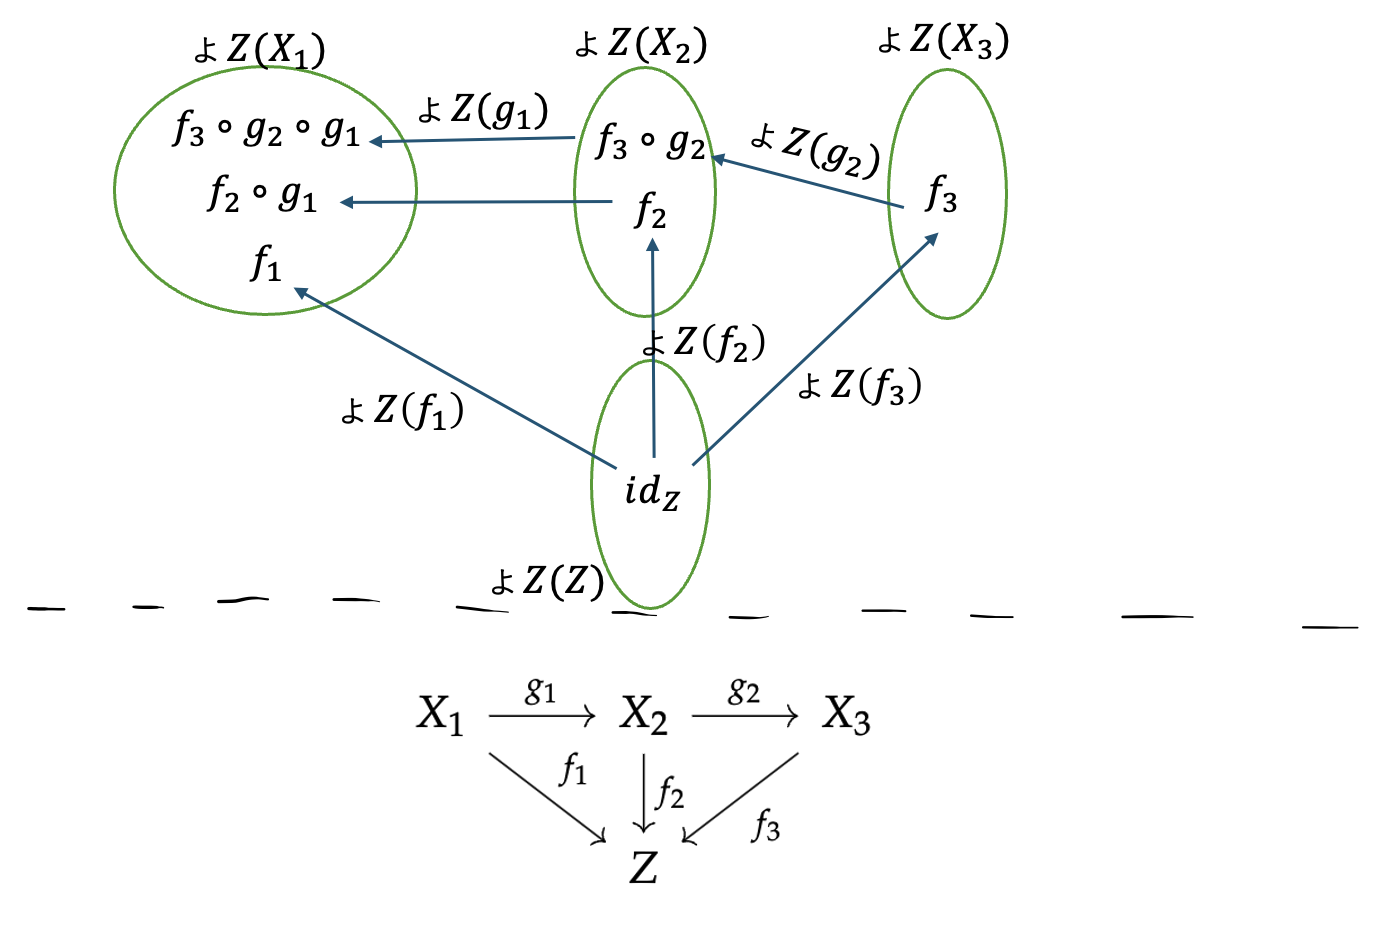
\includegraphics[width=300px]{fig/yo-1.png}
\end{center}

To build intuition, you should think of $\yo Z$ as describing ``the perspective
every other object in $\calC$ has on $Z$.'' Unpacking this more:
\begin{itemize}
  \item Let's look at the action of $\yo Z$ on $Z$ first.
  Unfolding the definition, we have:
  \begin{align*}
    (\yo Z)(Z) = \calC(Z, Z) = \{\id_Z\}
  \end{align*}
  So, somewhat vacuously, we might say: ``the perspective $Z$ has on itself 
  is the identity morphism''.
  And, for $X_1$, we have:
  \begin{align*}
    (\yo Z)(X_1) = \calC(X_1, Z) = \{f_1, f_2 \circ g_1, f_3 \circ g_2 \circ g_1 \}
  \end{align*}
  This is slightly more interesting: we would say, ``the perspective $X_1$ 
  has on $Z$ is through the $f_1$ morphism.''
  \item Now let's look at the action on morphisms. These will correspond 
  to ``changes in perspective''. Let's examine the action of $\yo Z$ 
  on the morphism $f_1$:
  \begin{align*}
    (\yo Z)(f_1 : X_1 \to Z) &: \yo Z \to \yo X_1\\
    &= \id_Z \mapsto \id_z \circ f_1 = f_1
  \end{align*}
  One can understand this as: ``to move from ``$X_1$'s perspective on $Z$ 
  to $Z$'s perspective on $Z$, follow the $f_1$ morphism''. Somewhat 
  more interestingly, we can also shift perspectives between $X_1$
  and $X_2$ via the $g_1$ morphism:
  \begin{align*}
    (\yo Z)(g_1 : X_1 \to X_2) &: (\yo Z)(X_2) \to (\yo Z)(X_1)\\
    &=
    \begin{cases}
      f_2 \mapsto f_2 \circ g_1 \\
      f_3 \circ g_2 \mapsto f_3 \circ g_2 \circ g_1
    \end{cases}
  \end{align*}
\end{itemize}

\subsection{Representables in the divisibility category}

\subsection{Representables in STLC}

\section{Representability}

\begin{definition}[Isomorphism of $\calC$-indexed sets]
  Two \(\calC\)-indexed sets \(P,Q\)
  are \emph{isomorphic}
if there are \(\calC\)-indexed functions \(\alpha : P \Rightarrow Q\)
and \(\beta : Q \Rightarrow P\)
such that \(\alpha\circ\beta=\idt_Q\) and \(\beta\circ\alpha=\idt_P\).
\end{definition}

\begin{definition}[Representability]
  \sloppy
  A \(\calC\)-indexed set \(P\) is \emph{representable}
  if there is an isomorphism \(\alpha : P \cong \yo X : \beta\)
  for some object \(X\) of \(\calC\).
\end{definition}

\begin{proposition}
  The \(\FinSet\)-indexed set \(\yo X \times \yo Y\)
  is representable.
\end{proposition}
\begin{proof}
  for any finite set \(A\), there is an isomorphism of sets
  \[
  \alpha_A : \FinSet(A,X \times Y) \cong \FinSet(A,X) \times \FinSet(A,Y).
  \]
  Concretely, \(\alpha_A\) is the function that sends
  a \(f \in \FinSet(A,X\times Y)\) to \((\pi_1 \circ f ,\pi_2,\circ f): \FinSet(A,X) \times \FinSet(A,Y) \).
  Its inverse is defined by \(\beta_A(f,g) = \angled{f,g}\).
  Both \(\alpha\) and \(\beta\) can be checked satisfy the naturality condition.
  Thus \(X\times Y\) represents \(\yo X \times \yo Y\).
\end{proof}

\begin{theorem}
  An object $P$ is a product of $A$ and $B$ if and only if 
  it represents $\yo A \times \yo B$.
\end{theorem}

\section{The category of elements}

%% \section{$\calC$-indexed sets}

%% Let's begin by studying the category $\mathbb{N}^\infty$, the category
%% constructed from the preorder formed by the natural numbers extended by
%% infinity:

%% \begin{center}
%% \begin{tikzpicture}[
%% ]
%% % Objects (circles)
%% \node[minimum size=0.6cm] (o1) at (0,-1) {0};
%% \node[minimum size=0.6cm] (o2) at (1.5,-1) {1};
%% \node[minimum size=0.6cm] (o3) at (3,-1) {2};
%% \node (dots) at (4.2,-1) {$\cdots$};

%% % Arrows between objects
%% \draw[->] (o1) -- node[above] {$f$} (o2);
%% \draw[->] (o2) -- node[above] {$g$} (o3);
%% \draw[->] (o3) -- (dots);

%% \draw[->] (o1) edge[loop above] node[above] {$\id_0$} (o1);
%% \draw[->] (o2) edge[loop above] node[above] {$\id_1$} (o2);
%% \draw[->] (o3) edge[loop above] node[above] {$\id_2$} (o3);
%% \end{tikzpicture}
%% \end{center}

%% Given a category $\calC$, a $\calC$-indexed set associates each object of
%% a category with a set.
%% Let's consider a concrete $\calC$-indexed set called $F$.
%% We can draw $F$ as a ``balloon picture'' like this:

%% \begin{center}
%%   \includegraphics[width=175px]{fig/balloon-1.png}
%% \end{center}

%% Above each object is drawn a (in this case, finite) set.
%% $F_1$ is the set $\{a, b, c\}$, and $F_2$ is is the set
%% $\{d, e\}$.
%% In addition to associating each object with a set,
%% a $\calC$-indexed set also associates each morphism $X \mor{f} Y$
%% with a function $F_Y \to F_X$, which we can draw on the balloon
%% picture like so:

%% \begin{center}
%% \includegraphics[width=175px]{fig/balloon-2.png}
%% \end{center}

%% Intuitively, we can see that $F$ is describing a relation between two
%% categories: our category of interest $\calC$, and an ``external''
%% category of sets and functions. This relation is called a \textbf{functor}.
%% Functors have actions on objects

% \begin{tikzpicture}[
%   node distance=1.5cm,
%   morphism/.style={-Stealth, thick}
% ]

% % Top row of labels
% \node (v) at (0,2) {$v$};
% \node (c) at (3,2) {$c$};

% % Middle row
% \node (y) at (-1.5,1) {$y$};
% \node (w) at (0,1) {$w$};
% \node (a) at (3,1) {$a$};

% % Bottom row (just above the objects)
% \node (x) at (-1.5,0) {$x$};
% \node (h) at (0,0) {$h$};
% \node (b) at (3,0) {$b$};

% % Objects (circles)
% \node[circle, draw, minimum size=0.6cm] (o1) at (0,-1) {0};
% \node[circle, draw, minimum size=0.6cm] (o2) at (1.5,-1) {1};
% \node[circle, draw, minimum size=0.6cm] (o3) at (3,-1) {2};
% \node (dots) at (4.2,-1) {$\cdots$};

% % Arrows between objects
% \draw[morphism] (o1) -- (o2);
% \draw[morphism] (o2) -- (o3);
% \draw[morphism] (o3) -- (dots);

% \end{tikzpicture}




% \begin{center}
%  \begin{tikzpicture}[]

% % Objects
% \node (A) at (0,0) {$A$};
% \node (B) at (3,0) {$B$};
% \node (C) at (1.5,2.5) {$C$};

% % Identity morphisms (loops)
% \draw[->] (A) edge[loop left] node[left] {$\text{id}_A$} (A);
% \draw[->] (B) edge[loop right] node[right] {$\text{id}_B$} (B);
% \draw[->] (C) edge[loop above] node[above] {$\text{id}_C$} (C);

% % Morphisms between objects
% \draw[->] (A) -- node[below] {$f$} (B);
% \draw[->] (A) -- node[left] {$g$} (C);
% \draw[->] (C) -- node[right] {$h$} (B);
% \node[draw, fit=(A)(B)(C), inner sep=1cm, rectangle] {};
% \end{tikzpicture}
% \end{center}


%% Throughout this section we will work with an arbitrary category \(\calC\).

%% \begin{definition}[$\calC$-indexed set]
%%   A $\calC$-indexed set is a functor $F : \calC^\text{op} \Rightarrow \Set$.
%% \end{definition}

%% \begin{example}
%%   Recall that \(\mathsf{STLC}\) is a category
%%   whose objects are types and whose morphisms \(A \to B\)
%%   are terms \(x : A \vdash M : B\) quotiented by \(\beta\eta\)-equivalence.
%%   For each type \(A\),
%%   the following defines a \(\mathsf{STLC}\)-indexed set \(\mathsf{Tm}(A)\):
%%   \begin{align}
%%   \mathsf{Tm}(B)(A) &= \text{the set of morphisms \(A\to B\)} \\
%%   \mathsf{Tm}(B)(N : A'\to A)
%%   &= (x\ofty A \vdash M : B) \mapsto (x'\ofty A' \vdash M[N/x] : B)
%%   \end{align}
%% \end{example}
%% This example is a special case of a canonical kind of \(\calC\)-indexed set.
%% \begin{definition}
%%   The \emph{representable \(\calC\)-indexed set at \(X\)}
%%   is written \(\yo X\) and defined by
%%   \begin{align}
%%     (\yo X)(A) &= \text{the set of morphisms \(A \to X\)} \\
%%     (\yo X)(A)(s : A' \to A) &= (f : A \to X) \mapsto (f \circ s : A' \to X)
%%   \end{align}
%% \end{definition}

%% \begin{definition}
%%   \sloppy
%%   Let \(P\) and \(Q\) be \(\calC\)-indexed sets.
%%   A \emph{\(\calC\)-indexed function}
%%   from \(P\) to \(Q\),
%%   written \(\alpha : P \Rightarrow Q\),
%%   is a family of functions \(\alpha_X : PX \to QX\)
%%   that ``respects substitution''
%%   in the sense that \(\alpha_{X'}(x\cdot_P p) = \alpha_X(x)\cdot_p p\).
%% \end{definition}

%% \begin{itemize}
%% \item \(\calC\)-indexed functions can be composed:
%%   the composition of \(\alpha : Q \Rightarrow R\)
%%   and \(\beta: P \Rightarrow Q\),
%%   written \(\alpha\circ\beta : P \Rightarrow R\),
%%   is defined by \((\alpha\circ\beta)_X = \alpha_X \circ \beta_X\).
%% \item For each \(\calC\)-indexed set \(P\),
%%   there is a \(\calC\)-indexed function \(\idt_P : P \Rightarrow P\)
%%   defined by \(\idt_{P,X} = \left(PX \xrightarrow{\idt_{PX}} PX\right)\).
%% \end{itemize}
%% By now you may have noticed that \(\calC\)-indexed sets and functions
%% look like they ought to form a category. More on this later.

%% \begin{definition}
%%   Two \(\calC\)-indexed sets \(P,Q\)
%%   are \emph{isomorphic}
%% if there are \(\calC\)-indexed functions \(\alpha : P \Rightarrow Q\)
%% and \(\beta : Q \Rightarrow P\)
%% such that \(\alpha\circ\beta=\idt_Q\) and \(\beta\circ\alpha=\idt_P\).
%% \end{definition}

%% \begin{definition}
%%   A \(\calC\)-indexed set \(P\) is \emph{representable}
%%   if there is an isomorphism \(\alpha : P \cong \yo X : \beta\)
%%   for some object \(X\) of \(\calC\).
%% \end{definition}


\chapter{Yoneda IV: universal constructions, elements, and properties}

\begin{definition}
  \sloppy
  Given two \(\calC\)-indexed sets \(P\) and \(Q\),
  their \emph{product} \(P\times Q\)
  is the \(\calC\)-indexed set defined by
  \((P\times Q)(X) = P(X)\times Q(X)\),
  with substitution defined by
  \((x,y)\cdot_{P\times Q} p = (x\cdot_P p, y\cdot_Q p)\).
\end{definition}

\begin{proposition}
  Let \(X\) and \(Y\) be two objects of a category \(\calC\).
  An object \(P\) is a product of \(X\) and \(Y\)
  if and only if \(\yo P\) is isomorphic to \(\yo X \times \yo Y\).
\end{proposition}

\begin{definition}
  Given two objects \(X\) and \(Y\) of a category \(\calC\),
  there is a \(\calC\)-indexed set of \emph{closures},
  written \(\mathsf{Clos}(X,Y)\),
  defined by \(\mathsf{Clos}(X,Y)(\Gamma) = \calC(\Gamma\times X, Y)\),
  with substitution defined by
  \[
    \mathsf{Clos}(X,Y)(s : \Gamma'\to \Gamma)(f : \Gamma\times X \to Y)
    = \angled{\gamma',x} \mapsto f \circ \angled{s\circ \gamma', x}
  \]
  on generalized elements.
\end{definition}

\begin{proposition}
  Let \(X\) and \(Y\) be two objects of a category \(\calC\).
  An object \(E\) is the exponential \(Y^X\)
  if and only if \(\yo E\) is isomorphic to \(\mathsf{Clos}(X,Y)\).
\end{proposition}

\begin{proposition}
  Suppose the \(\calC\)-indexed set \(P\) is represented
  by the object \(X\).
  Then there exists an element \(u \in PX\),
  called the \emph{\(P\)-universal element},
  which satisfies the following \emph{universal property}:
  for any object \(\Gamma\) and any element \(g \in P\Gamma\),
  there exists a unique morphism \(\hat g : \Gamma \to X\)
  such that \(g = u \cdot_P \hat g\).
\end{proposition}

\begin{itemize}
\item In the case of the product, with \(\yo P \cong \yo X \times \yo Y\),
  the universal element is an element \(u \in \calC(P,X) \times \calC(P,Y)\),
  which is a pair of morphisms \(P\to X, P\to Y\).
  The universal property of this pair is that any other pair \(\Gamma \to X,\Gamma\to Y\)
  factors uniquely through it---precisely the universal property of products
\item In the case of exponents, with \(\yo E \cong \calC(A\times(-),B)\),
  the universal element is an element \(u \in \calC(A \times E,B)\),
  which is a morphism \(A \times E \to B\).
  The universal property of this morphism is that any other morphism
  \(A \times \Gamma \to B\)
  factors uniquely through it---precisely the universal property of exponents.
\end{itemize}

\chapter{Yoneda IV}

%% - Grothendieck universes
%% - The category Set
%% - Functors; opposite categories; C-indexed sets as functors
%% - Natural transformations; C-indexed functions as natural transformations
%% - The Yoneda lemma (without showing naturality in P,c)

%% \begin{itemize}
%% \item Functors form a category where morphisms are natural transformations \begin{itemize}
%%     \item Natural transformations as homotopies between diagrams
%%       (the \(C\to D^\to\) example revisited)
%%     \item Natural transformations as polymorphic maps
%%   \end{itemize}
%% \item Definition of Yoneda embedding
%% \item Restatement of universal properties from previous week in terms of Yoneda embedding
%% (e.g., for products, \(\yo(a\times b) \cong \yo(a)\times \yo(b)\).)
%% \item Yoneda embedding full and faithful. Use this to quickly prove some basic facts:
%%   associativity and commutativity of sums and products, distributivity of products over sums,
%%   ...
%%   These imply type isomorphisms in STLC and Set, entailments of propositional logic.
%% \item Yoneda preserves limits.
%%   This gives a quick proof that all limits can be constructed from products and equalizers.
%%   From this we can compute limits in STLC (it won't have all of them
%%   but it will have some).
%% \end{itemize}

%% \todo: \begin{itemize}
%% \item Slice over c is category of elements of yo c
%% \end{itemize}
